\chapter{Parallel iterations (temporary title)}

\todo{partie synchrone et partie asynchrone}

\section{Introduction}

Parallel Iterative Algorithms (PIA) are always designed to harness the system on which they are running, and the main behavior control on those algorithms is their flow control of computation and communication tasks. Computation tasks involved all the operations done by the process unit whereas communications tasks implies the exchange of data between different computing unit. Base on those two key criteria, we can define a classification with four main classes for PIA : Synchronous Iteration and Synchronous Communication (SISC), Synchronous Iteration and Asynchronous Communication (SIAC), Asynchronous Iteration and Synchronous Communication (AISC) and lastly Asynchronous Iteration and Asynchronous Communication. All those models expect the AISC model, are worth exploring in terms of behavior in order to highlight the best systems where their performance are at their peak.
In this chapter, we will explore those classes, and then pinpoint a key aspect of all those algorithm: the convergence detection.



\section{SISC model}

[talk about convergence condition maybe with references]
Synchronous Iteration and Synchronous communication model for parellisation is the most used parallelization technique due to its intuitiveness. In fact the model is not so different from its sequential counterpart. While in the sequential algorithm, only one computing unit is at work, here the main task is divided in sub-tasks assigned to different computing units, all of them connected to each other by a network in order to exchange data dependencies. This model implies that all the computing units should be at the same iteration k (k element de 0 à n)  at time t (t << infini) , and data exchange mostly happened at the end of iteration k. In figure~\ref{fig:SISC}, each iteration is represented by a grey square and the arrows are the communication happening between computing unit.


\begin{figure}[htbp]
	\centering
	\captionsetup{justification=centering}
	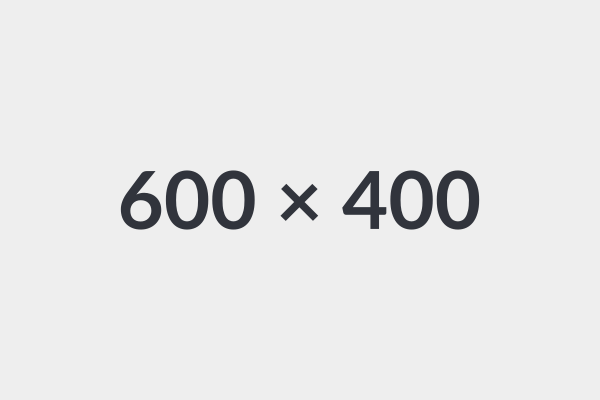
\includegraphics[height=2.5in]{images/placeholder.png}
	\caption{Synchronous Iteration and Synchronous Communication}
    \label{fig:SISC}
\end{figure}

This model appears to be well suited for parallel machines where all the computing units are of the same computing power, receive the same workload and the inter-communication between those computing units is a high speed connection. No idle time is expected in these conditions. Meanwhile, when  faced with an heterogeneous environment ( hardware and network heterogeneity),  this model can perform poorly. Notably, the first problem is the difference of computing power in the environment implying that with the same workload, computing units with more computing power will end their sub-task as quickly as they can while those with less power will take more time. This induce some idle time as some computing units despite having send their data to others, need to wait to receive the data corresponding to iteration k. Furthermore, computing units can be connected with different types of network showing different bandwidth, latency …. This add more idle time as data is not transmitted at the same speed.  To sum up, the SISC model is not expected to perform well on systems like local clusters or distributed systems that often rely on heterogeneous infrastructures and furthermore, not good for large problems. A workaround could be to minimize the idle time by overlapping computations and communication. 

\section{SIAC model}

[talk about convergence condition maybe with references]
The SIAC model rely on a subtle workaround despite being really close to the SISC and sequential scheme. In fact this model suggests the asynchronicity of communication, meaning that the computations and communication can be overlap. Given a set of data dependency, as soon as part of this data is computed on one computing unit, it's send to other computing units, then the computation should progress to complete the computation of all data dependencies. It's worth noting that the sending operation is not blocking, only the receiving operation is blocking in order to make sure that each process unit possess all data needed for the next iteration. [The effect of high latency network is diminished ]. Consequently, the idle time is minimize even though not suppress. As mentionned earlier, given the same distributed workload the most computational powered computing unit steal needs to wait for other non powerful computing units to compute all their data and send them before moving to the next iteration. Figure~\ref{fig:SIAC} illustrate this behavior.


\begin{figure}[htbp]
	\centering
	\captionsetup{justification=centering}
	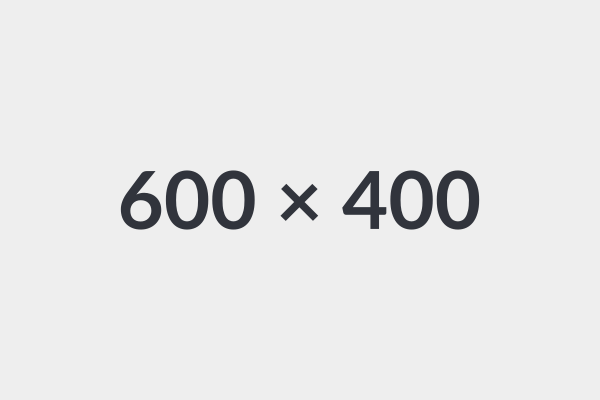
\includegraphics[height=2.5in]{images/placeholder.png}
	\caption{Synchronous Iteration and Aynchronous Communication}
    \label{fig:SIAC}
\end{figure}

To sum up, even though the idle time is minimize, it is not zeroed by this mechanism of asynchronous communication. The same assumptions hold for this scheme as far as distributed system is concerned: SIAC is need another level of asynchrony to fully harness the infrastructure.


\section{AIAC model}

[ajouter ici que le nombre d'iterations peut augmenter pour l'obtention de la convergence, mais que cette augmentation vaut mieux que le retard accusé par les systems synchrones, surtout dans des environnements ou le reseau est très congestionné ou defaillant]
The asynchronous iteration and asynchronous communication scheme also called the asynchronous iteration model is the global behavior of an algorithm that does not need any synchronization step whether at the iteration level of communication level, iterations and communication are all asynchronous. Rather than waiting for updates like in previous schemes, the computing unit just keep working with the last updates it receives, until new data arrive asynchronously to be consumed. In this context, the previously mentioned idle time is completely suppressed as shown by figure~\ref{fig:AIAC}


\begin{figure}[htbp]
	\centering
	\captionsetup{justification=centering}
	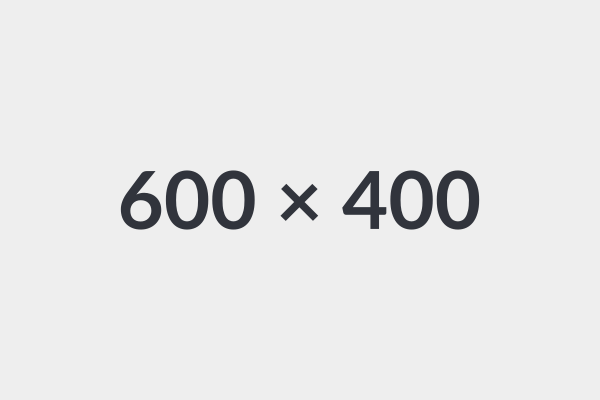
\includegraphics[height=2.5in]{images/placeholder.png}
	\caption{Aynchronous Iteration and Aynchronous Communication}
    \label{fig:AIAC}
\end{figure}

Assuming communications are now asynchronous and consequently free to be performed at any level of the algorithm, one can legitimately ask for performances purposes, when, where to send or receive data, and how to group data for efficient communication. Theses questions lead to a practical classification of AIAC algorithms in two classes: Semi-flexible communication AIAC and flexible communication AIAC models.

\subsubsection{Semi-flexible communication}


Semi-flexible communication refers to AIAC algorithms that has some restrictions over communication behavior, whether on the sender computing unit or on the receiver computing unit. This difference actually leads to two distincts sub-classes:


\begin{description}

    \item[Sender-side semi-flexibility] As the sub-class name suggests, the communication restrictions operate on the sender side. On the receiver side, no changes is to be noted. The receiver computing unit receives the updates during the iteration or at the end of the iteration, but only integrates the new data during the next iteration. On the sender side, the updates are sent as soon as the are available, preferably by group of data, to avoid network congestion. The ultimate goal of this scheme is to speed up the convergence process. Figure~\ref{fig:AIAC-sender-semi-flexible} illustrate this behavior.
    
    \item[Receiver-side semi-flexibility] Conversely to the previous sub-class, it’s the sender that does keep a rigid behavior and the receiver that has a flexible one. In fact the sender only send all the data necessary for updates at the end of every iteration. On the receiver side, the data reception is done as soon as the update is available, and the new data is integrated in the process of the computation on the same iteration if possible.Figure~\ref{fig:AIAC-receiver-semi-flexible} illustrate this behavior.
\end{description}


\begin{figure}[htbp]
	\centering
	\captionsetup{justification=centering}
	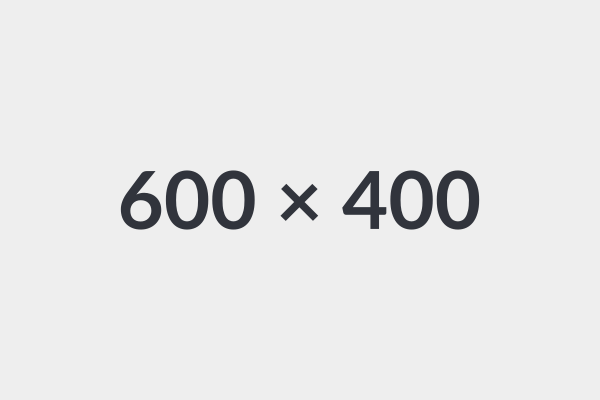
\includegraphics[height=2.5in]{images/placeholder.png}
	\caption{Sender-side semi-flexibility}
    \label{fig:AIAC-sender-semi-flexible}
\end{figure}


\begin{figure}[htbp]
	\centering
	\captionsetup{justification=centering}
	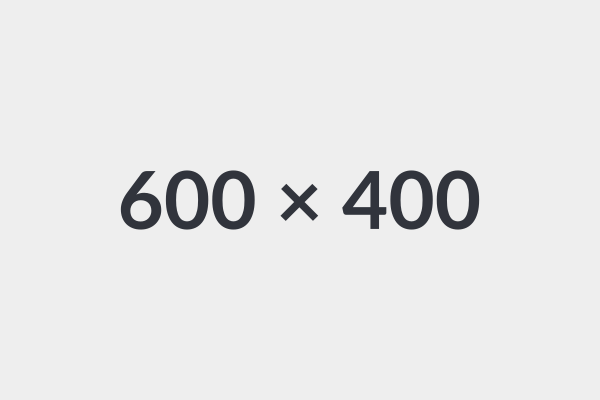
\includegraphics[height=2.5in]{images/placeholder.png}
	\caption{Receiver-side semi-flexibility}
    \label{fig:AIAC-receiver-semi-flexible}
\end{figure}


\subsubsection{Flexible communication}

The flexible communication scheme allow every computing unit to send data dependencies as soon as available on the sender side, and the on the receiver side, receive and integrate in the same iterations the new data available.Figure~\ref{fig:AIAC-flexible} illustrates this behavior.


\begin{figure}[htbp]
	\centering
	\captionsetup{justification=centering}
	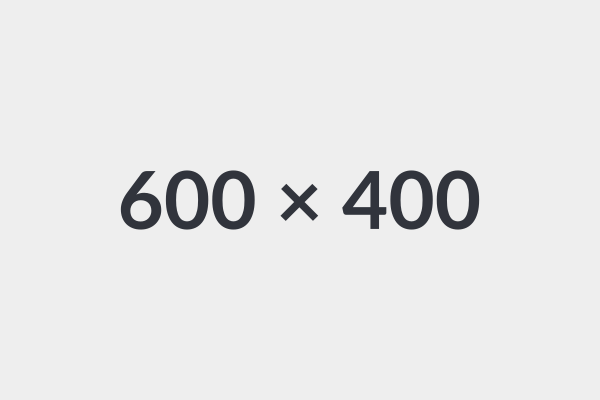
\includegraphics[height=2.5in]{images/placeholder.png}
	\caption{Receiver-side semi-flexibility}
    \label{fig:AIAC-flexible}
\end{figure}

\section{Convergence conditions and detection}


\todo{detection de convergence centralisé classique + detection de convergence distributé comme dans le livre}

\section{Programming environments}
\subsection{Dedicated programming environments}
\subsection{Non-dedicated programming environments}


\section{Conclusion}